% !TEX root = ../../Tesi_Triennale_PMNS.tex
\chapter[Segnali di GW da BNS]{Segnali di onde gravitazionali da BNS}
\label{chapter:segnaleGWdaBNS}
Una stella di neutroni è la fase finale dell'evoluzione stellare, che segue alla cessazione delle reazioni di fusione nucleare degli elementi leggeri al suo interno, per stelle con massa tale che
\begin{equation}
   	\SI{10}{\solarmass} < M < \SI{25}{\solarmass}
   	\label{eqn:massNS}
\end{equation}
Accade dunque che, in una certa fase del collasso, le densità estremamente alte possono portare gli elettroni a interagire con i protoni, attraverso il fenomeno della cattura elettronica, portando alla formazione di neutroni (e neutrini). Date le densità estreme della stella di neutroni, rimane incertezza sulle equazioni di stato della materia.\cite{hobson2006general}

Una stella di neutroni (NS) è resa stabile, contro il collasso dovuto alla forza di gravità, non da pressioni termiche come per il sole, ma da forze legate al principio di esclusione di Pauli e interazioni nucleari tra i neutroni. Queste forze hanno effetti solo sopra le densità nucleari, che spiega perché le NS sono sono così compatte (una NS ha una massa poco superiore rispetto alla massa solare in un raggio di $\smallsim$10 km)\cite{hartle2003gravity}
%    ALTRO?
\begin{wrapfigure}{r}{0.45\textwidth}
	\vspace{-15pt}
	\begin{center}
		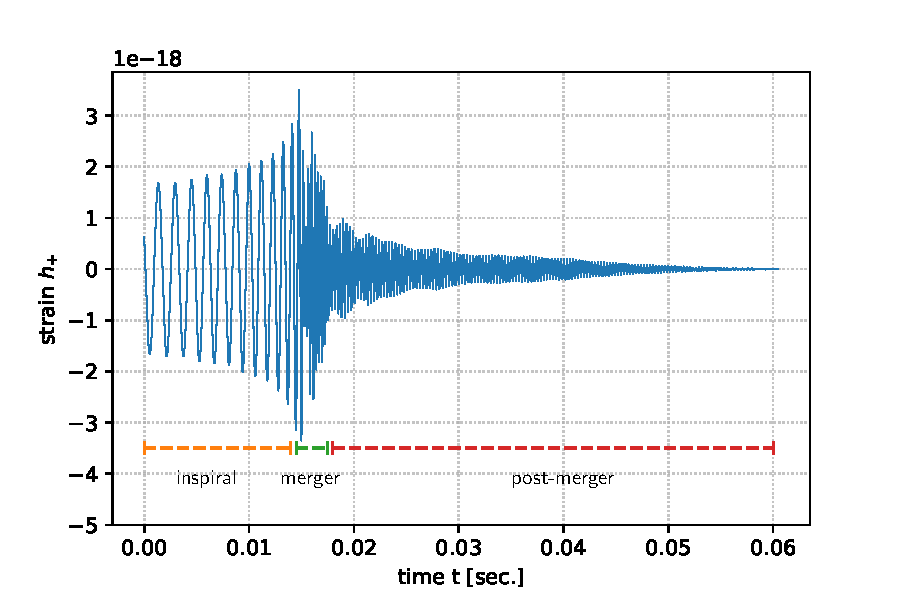
\includegraphics[width=0.5\textwidth]{figures/Capitolo_1/APR4.pdf}
	\end{center}
	\vspace{-10pt}
	\caption{Forma d'onda per la coalescenza di una BNS con equazione di stato APR4, con una divisione qualitativa tra le diverse fasi}
	\label{fig:forma_onda_APR4}
	\vspace{-10pt}
\end{wrapfigure}
Un sistema binario di stelle di neutroni (BNS), ovvero una coppia di NS che, legato attraverso la forza di attrazione gravitazionale, ruota attorno al centro di massa, emette segnali di onda gravitazionale (GW) che possono essere interpretati come fase di inspiral, merger e post-merger.

La lunga fase di spiraleggiamento consiste nelle due stelle che ruotano attorno al centro di massa, a causa dell'emissione di energia sotto forma di onde gravitazionali, il raggio delle orbite diminuisce portando ad un incremento in ampiezza e frequenza della GW, producendo il caratteristico "chirp". Questa è l'unica fase che viene descritta con un approccio analitico.

La fase di spiraleggiamento termina con i due oggetti che si scontrano dando inizio alla fase di merger e quindi, dopo la fusione, al post-merger, che in base alle proprietà iniziali del sistema può portare a forme d'onda e oggetti diversi.	Mentre la fase di merger dura pochi millisecondi, la fase di post-merger genera un segnale quasi-stazionario. Queste due fasi risultano più complesse da modellare, per cui per il loro studio si fa affidamento a metodi numerici. \cite{maggiore2008gravitational}

\section[Frequenze caratteristiche]{Frequenze caratteristiche di merger e post-merger}
\label{section:frequenze_caratteristiche}
Una BNS realistica presenta una massa compresa tra $\smallsim\SI{2.4}{\solarmass}$ e $\smallsim\SI{2.8}{\solarmass}$ e una differenza tra le due componenti che è di $\smallsim20\%$ o minore. 
A partire dal segnale di GW, in particolare nelle fasi di merger e post-merger, possono essere ottenute informazioni sull'equazione di stato della materia a densità nucleari e, da un'analisi spettrale, informazioni sulla tidal deformability (deformabilità mareale) delle due stelle.

Osservando dunque lo spettro del segnale di onda gravitazionale nella fase di merger, in particolare per binarie con masse che non differiscono per più del 20\%, questo presenterà alcune proprietà\cite{Rezzolla_2016}:
\begin{wrapfigure}{r}{0.45\textwidth}
	\vspace{-5pt}
	\begin{center}
		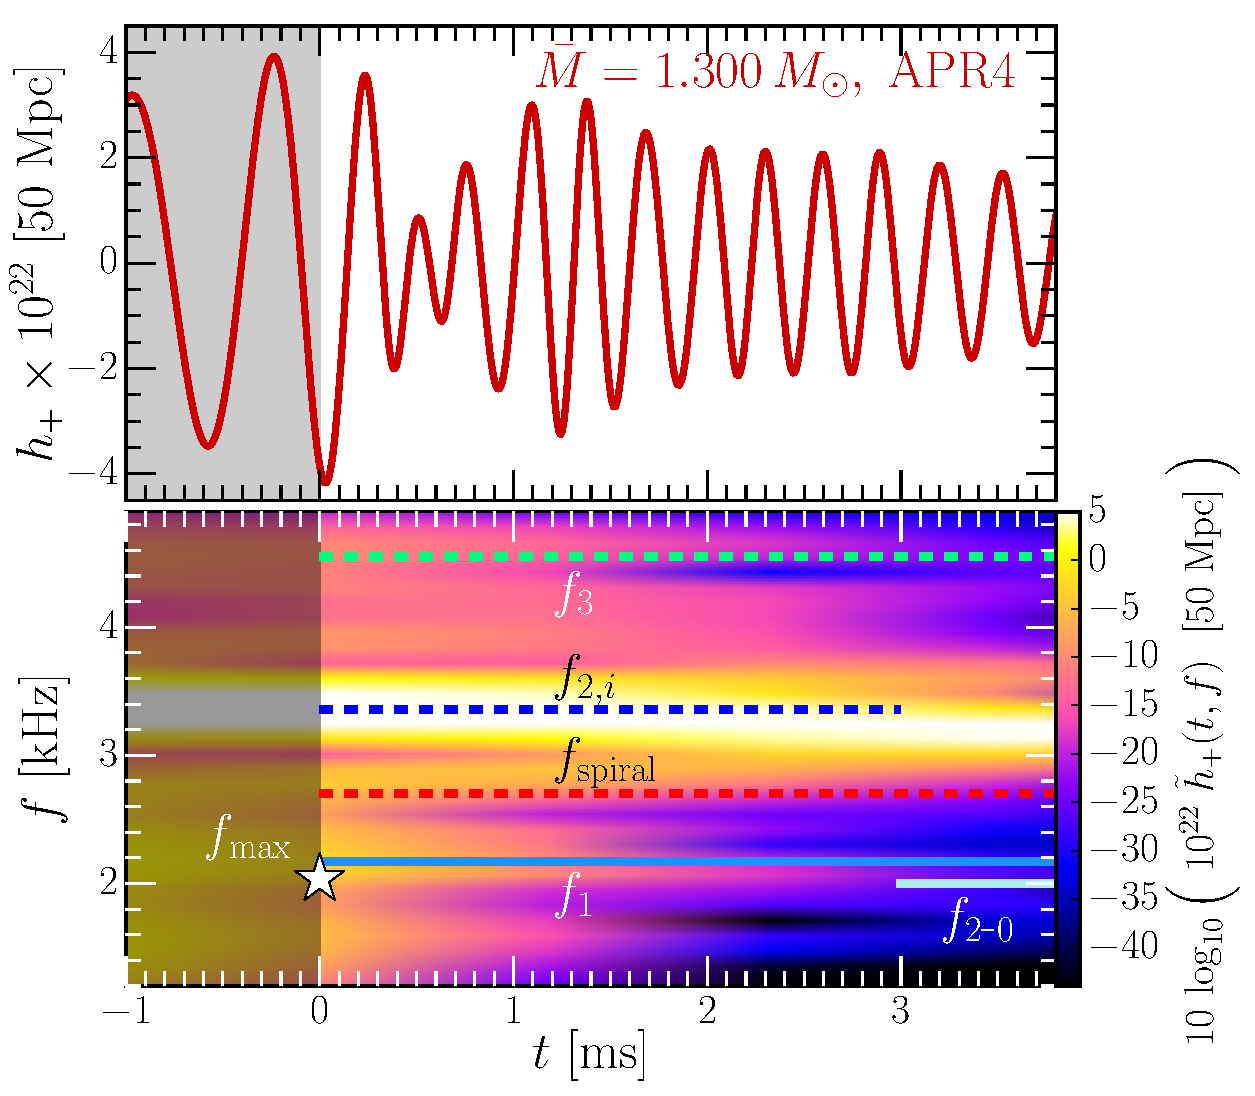
\includegraphics[width=0.5\textwidth]{figures/Capitolo_1/GW_spectrogram_short_APR4-q10-M1300.pdf}
	\end{center}
	\vspace{-10pt}
	\caption{Forma d'onda e relativo spettrogramma per il merger di una BNS con equazione di stato APR4 (morbida), presa da \cite{Rezzolla_2016}}
	\label{fig:spettrogramma_merger_APR4}
	\vspace{-25pt}
\end{wrapfigure}
\begin{itemize}
   	\item la frequenza della GW al massimo di ampiezza $f_{max}$ è legata in modo quasi-universale con la tidal deformability delle due stelle;
   	\item le frequenze $f_1$, $f_{2,i}$ e $f_3$ rappresentano i picchi principali visibili dall'osservazione del post-merger, tra le quali si ottiene la seguente relazione empirica:
   	\begin{equation}
   		f_{2,i}\simeq\frac{f_1 + f_3}{2} 
   		\label{eqn:f1_2_3}
   	\end{equation} 
   	il picco $f_1$ è legato alla compattezza delle stelle, mentre il picco $f_{2,i}$ è legato al raggio della configurazione non rotante più massiva e corrisponde al modo fondamentale della NS ipermassiva con l=2=m;
   	\item si identifica in alcuni casi un altro picco $f_{2-0}$ che si riferisce all'accoppiamento tra il modo fondamentale con l=2=m e il modo con simmetria assiale, cioè con l=2 e m=0;
\end{itemize}
   
\begin{itemize}
   	\item il picco $f_{spiral}$ associato alla deformazione spiraleggiante dovuta alla rotazione, è però impossibile da misurare in calcoli numerici e si utilizzano dunque i valori prodotti da considerazioni analitiche. Si nota infine che $f_{spiral}$ coincide per molte EOS (in particolare EOS rigide) con la frequenza $f_1$, mentre per altre (EOS morbide) non si ha questa corrispondenza.
\end{itemize}
%	FORSE UN PO' CONFUSO

\begin{wrapfigure}{r}{0.45\textwidth}
	\vspace{-10pt}
	\begin{center}
		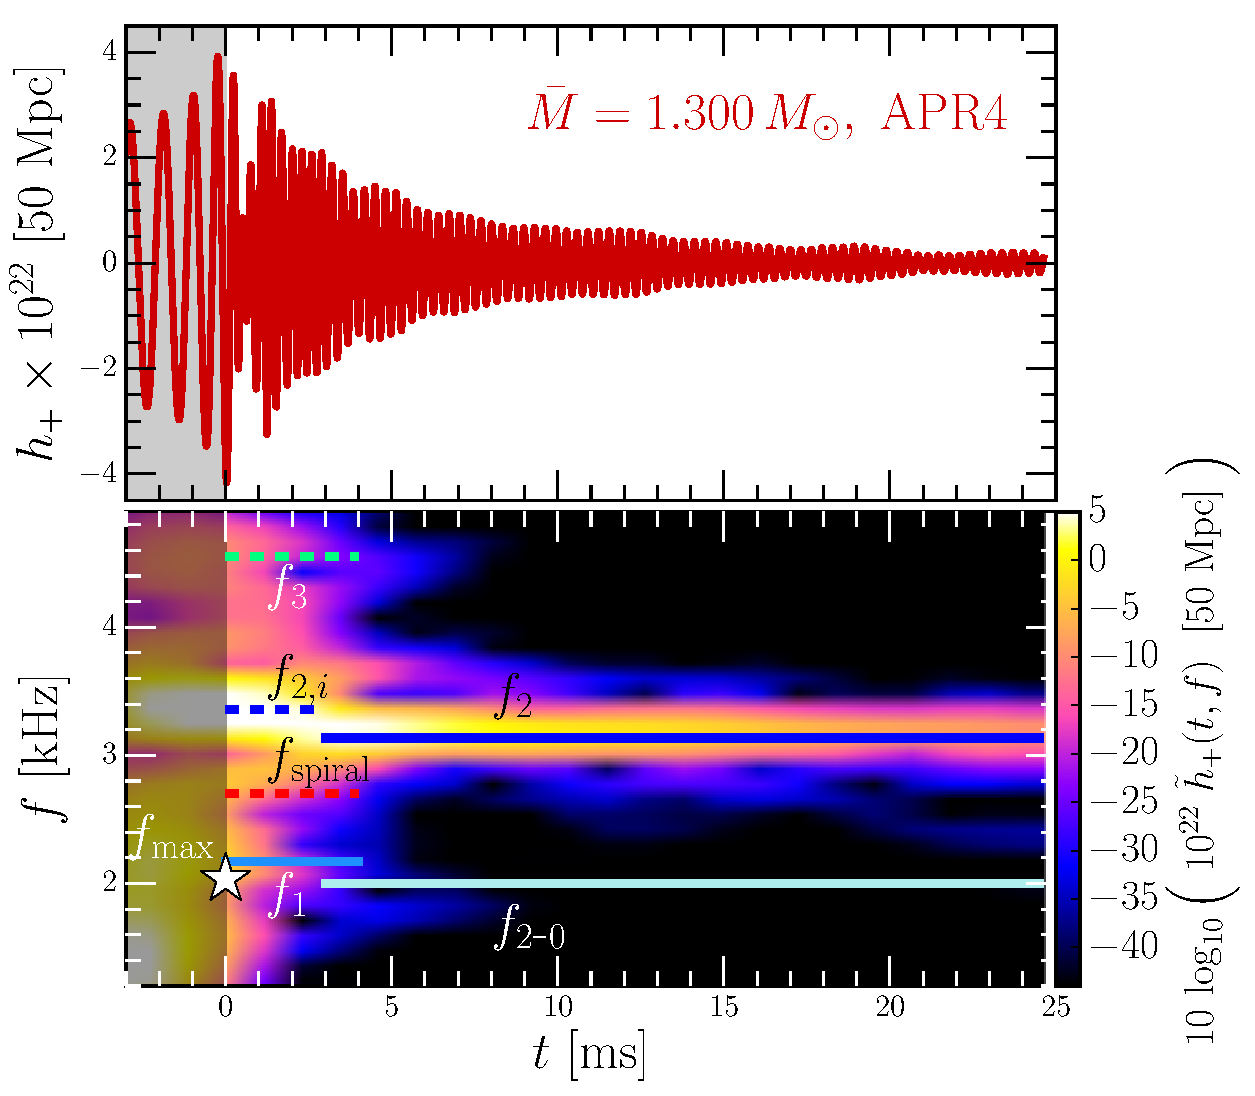
\includegraphics[width=0.5\textwidth]{figures/Capitolo_1/GW_spectrogram_APR4-q10-M1300.pdf}
	\end{center}
	\vspace{-10pt}
	\caption{Forma d'onda e relativo spettrogramma per il post-merger di una BNS con equazione di stato APR4, presa da \cite{Rezzolla_2016}}
	\label{fig:spettrogramma_postmerger_APR4}
	\vspace{-50pt}
\end{wrapfigure}

Nella fase di post-merger, nei casi in cui il sistema non collassa immediatamente in un buco nero, evidenziando nella forma d'onda una fase di ringdown in cui il segnale si spegne, l'unica frequenza a sopravvivere è il picco $f_2$, spariscono gli altri picchi, lasciando solo $f_{2-0}$ a basse energie.

È poi possibile trovare diverse relazioni quantitative che legano le frequenze osservate con le proprietà stellari, che risultano particolarmente utili come verifica delle previsioni teoriche.

%    Cenno sulle equazioni di stato.
\section{Oggetto residuo}
\label{section:residual}
Ci sono quattro possibili risultati della coalescenza di due stelle di neutroni, in base alle masse delle stelle e dalle loro equazioni di stato. 
Data la massa dell'oggetto residuo $M$, facendo riferimento alla figura \ref{fig:EvoluzioneBNS}:

\begin{itemize}
	\item $M\gtrsim 1.5 M_{TOV}$\footnote{$M_{TOV}$ è detta massa di Tolman-Oppenheimer-Volkoff e indica la massa massima che può avere una stella di neutroni non rotante}: il sistema collassa immediatamente in un buco nero seguendo il percorso A$\rightarrow$ B$\rightarrow$ C;
\end{itemize}

\begin{itemize}
	\item $1.2 M_{TOV} \lesssim M \lesssim 1.5 M_{TOV}$: l'oggetto rimanente è una stella di neutroni ipermassiva, che collassa in un buco nero in un tempo $\lesssim 1$s, seguendo A$\rightarrow$ B$\rightarrow$ D$\rightarrow$ E;		
	\item $M_{TOV} \lesssim M \lesssim 1.2 M_{TOV}$: rimane una stella di neutroni supermassiva che è destinata a collassare in un buco nero in un tempo di 10 \textdiv $10^4$s, secondo il percorso A$\rightarrow$ B$\rightarrow$ D$\rightarrow$ F$\rightarrow$ G;		\item $M\lesssim M_{TOV}$: rimane una stella di neutroni stabile, secondo il percorso A$\rightarrow$ B$\rightarrow$ D$\rightarrow$ F$\rightarrow$ H \cite{sarin2020evolution}.	
\end{itemize}

\vspace{-20pt}
\begin{SCfigure}[][h]
	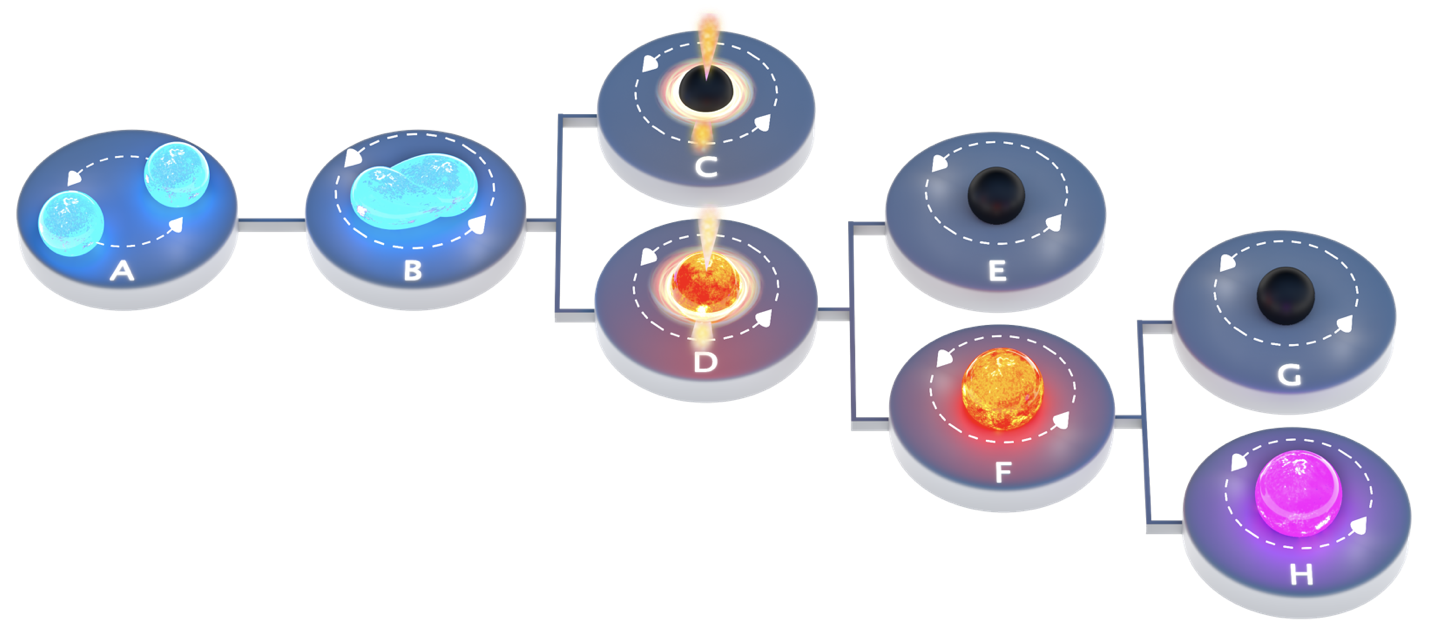
\includegraphics[scale=0.25]{figures/Capitolo_1/MagnetarEvolution.png}
	\captionsetup{width=0.8\textwidth}
	\caption{Rappresentazione pittorica del destino del residuo del merger di un sistema binario di stelle di neutroni, presa da \cite{sarin2020evolution}}
	\label{fig:EvoluzioneBNS}
	\vspace{-15pt}
\end{SCfigure}
%\begin{center}
%	\begin{figure}[ht]
%		\vspace{-20pt}
%		\centering
%		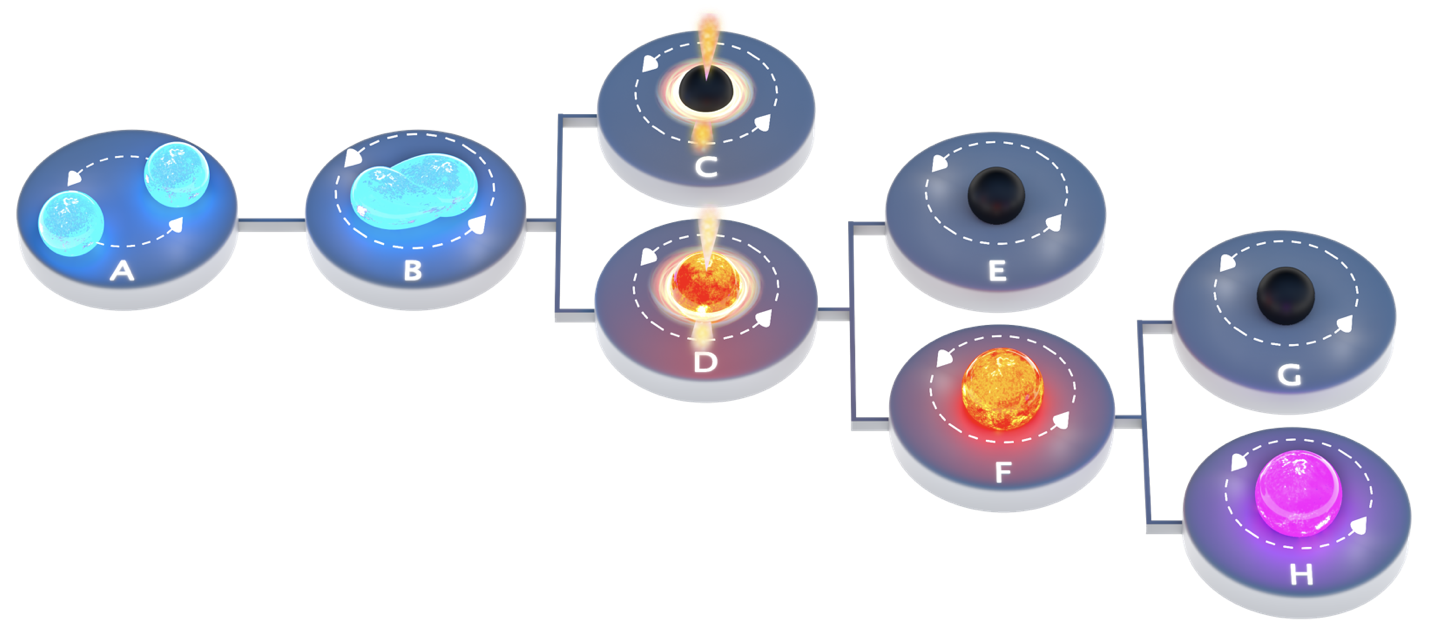
\includegraphics[scale=0.2, angle=0]{figures/Capitolo_1/MagnetarEvolution.png}
%		\setlength{\belowcaptionskip}{-25pt}
%		\caption{Rappresentazione pittorica del destino del residuo del merger di un sistema binario di stelle di neutroni, presa da \cite{sarin2020evolution}}
%		\label{fig:EvoluzioneBNS}
%	\end{figure}
%\end{center}
%Veloce descrizione delle possibili espulsioni di kilonovae

I sistemi binari di stelle di neutroni, oltre che ottime sorgenti di onde gravitazionali, risultano anche i migliori scenari per spiegare la fenomenologia dei lampi gamma brevi (short gamma ray burst). I lampi gamma consistono nell'emissione di intensi raggi gamma con uno spettro di durate estremamente vario, per cui si distinguono i short gamma ray burst con durata tipica inferiore a 2s e con un energia media dei fotoni superiore, i long gamma ray burst la quale durata è piccata attorno a 30s, fino agli ultra-long gamma ray burst che arrivano a durare diverse ore, mediamente meno energetici. 
La separazione è legata ai fenomeni fisici che generano questo fenomeno: mentre i GRB lunghi hanno origine nel collasso del nucleo di stelle massive, nel fenomeno della post-luminescenza, la comprensione dell'origine di GRB brevi è risultata più complessa, infatti l'osservazione sperimentale ha portato ad escludere il collasso di stelle massive come origine di tali fenomeni. Candidati plausibili sono risultati invece i merger di BNS o di binarie NS-BH, poiché la durata di GRB brevi richiede strutture compatte con caratteristiche sulla scala dei tempi nell'ordine delle decine di millisecondi, compatibilit con il merger di un sistema binario di compatte. In realtà l'osservazione sperimentale, in particolare di GW170817, evento che si approfondirà nel capitolo \ref{chapter:gw170817}, mostra come le caratteristiche dei GRB associati a questi fenomeni risultano differenti dai GRB cosmologici, per cui si ipotizza che questi siano espressione di un nuovo tipo di transiente \cite{maggiore2018gravitational}.

\begin{wrapfigure}{r}{0.45\textwidth}
	\vspace{-50pt}
	\begin{center}
		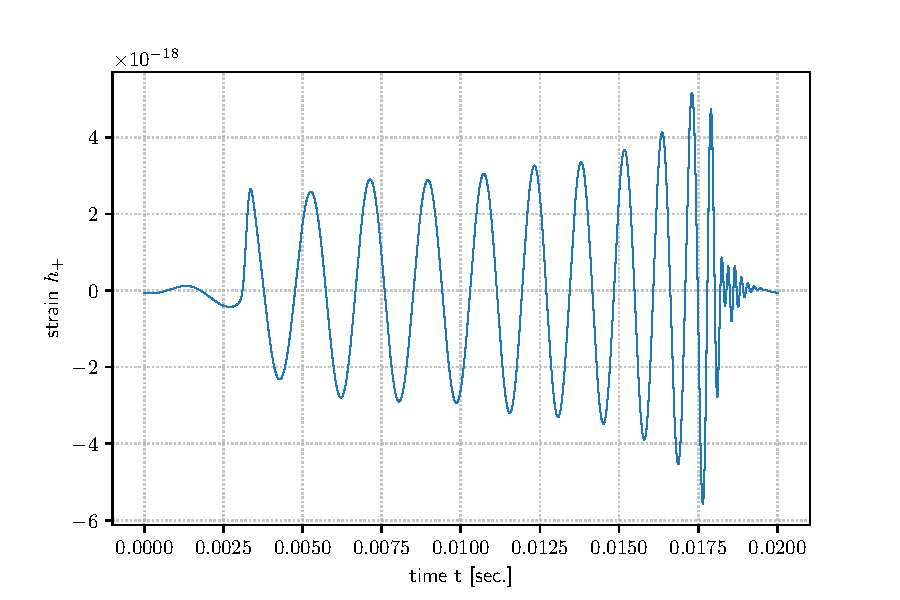
\includegraphics[width=0.5\textwidth]{figures/Capitolo_1/SHT2.2.pdf}
	\end{center}
	\vspace{-10pt}
	\caption{Forma d'onda per la coalescenza di una BNS con equazione di stato SHT2, in cui le masse sono tali da portare il sistema a collassare immediatamente in un BH, producendo nella fase di post merger il ringdown}
	\label{fig:FormaOndaBH}
	\vspace{-30pt}
\end{wrapfigure}
\subsection{Formazione diretta un black hole}	
\label{subsection:Diretto_Black_hole}

La formazione diretta di un buco nero dopo la coalescenza implica, come si osserva in figura \ref{fig:FormaOndaBH} lo spegnimento del segnale, con un collasso quasi sferico che genera delle onde gravitazionali minime\cite{sarin2020evolution}.

Questo tipo di segnale ha la particolarità, al contrario degli altri casi di post-merger, di ammattere uno studio analitico attraverso metodi perturbativi relativamente semplici (decrescita esponenziale con un tempo caratteristico legato alla massa del buco nero)\cite{maggiore2018gravitational}.

\subsection{Formazione di una NS ipermassiva}
\label{subsection:ipermassiva}	
La maggior parte dei merger di stelle di neutroni porta alla formazione di stelle di neutroni ipermassive, supermassive o stabili. 

Una stella di neutroni ipermassiva è tale da avere una massa superiore al massimo in massa per una stella rotante uniformemente $M_{TOV}$, ma non collassa per la rotazione differenziale, cioè il fenomeno per cui le sue diverse parti ruotano con velocità angolare differente che permette una maggiore stabilità rispetto a stelle non rotanti o rotanti uniformemente \cite{Baumgarte_2000}, e per il supporto di gradienti termici. Nel momento in cui la stella rallenta la sua rotazione e/o si raffredda il supporto alla sua stessa massa termina e la stella collassa in un buco nero. 
Nel caso in cui la stella ipermassiva abbia massa tale che $M \gtrsim 1.2 M_{TOV}$ la rotazione uniforme non può dare sufficiente supporto centrifugo per evitare il collasso, per cui la stella collassa non appena la rotazione differenziale termina.

È in generale molto complessa la fisica che regola il collasso dell'ipermassiva residua tuttavia assumendo che per il rilascio del lampo gamma sia necessario tale collasso in buco nero, il ritardo con il quale si è osservato per GW170817, come si vedrà nel capitolo \ref{chapter:gw170817}, può essere, almeno in parte, spiegato con il collasso.

\begin{wrapfigure}{r}{0.45\textwidth}
	\vspace{-20pt}
	\begin{center}
		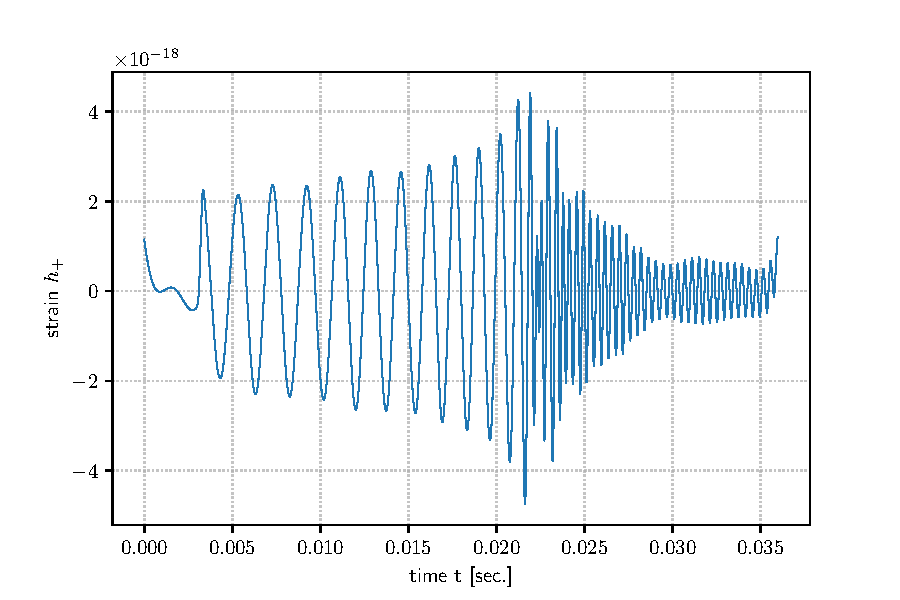
\includegraphics[width=0.5\textwidth]{figures/Capitolo_1/SHT2.0.pdf}
	\end{center}
	\vspace{-10pt}
	\caption{Forma d'onda per la coalescenza di una BNS con equazione di stato SHT2, in cui le masse sono tali da portare il sistema a formare una NS ipermassiva, producendo nella fase di post merger un segnale visibile}
	\label{fig:FormaOndaToNS}
	\vspace{-20pt}
\end{wrapfigure}

L'emissione di GW dalla fase di post-merger è attesa avere una ampiezza di strain relativamente ampia, confrontabile con il picco dell'inspiral ma a frequenze maggiori, in cui i detector hanno una precisione sensibilmente inferiore.

Simulazioni numeriche relativistiche di merger di BNS e l'evoluzione del post-merger mostra che l'emissione di GW da un residuo ipermassivo è dominato da modi-f quadrupolari, che in base alla EOS che si considera può trovarsi tra $\smallsim2$ e 4kHz, ed è fortemente correlato con la compattezza e la tidal deformability delle stelle. Questa correlazione, con quantità calcolate per stelle di neutroni fredde e non rotanti, stato in cui non si trova l'ipermassiva residua, suggerisce come gli effetti dovuti a rotazione e temperatura giocano un ruolo limitato nelle proprietà del segnale di onda gravitazionale e mostra come la misura del modo dominante nella frequenza del post-merger possa portare a una importante misura dell'equazione di stato nucleare\cite{sarin2020evolution}.

\subsection{Formazione di una NS con lunga vita media}
\label{subsection:long_lived}
I residui del post-merger che hanno una massa inferiore a $\smallsim1.2M_{TOV}$ sopravvivono per un tempo superiore al secondo e vengono denomiate supermassive se hanno una massa superiore al limite definito in precedenza $M_{TOV}$, mentre per valori inferiori sono stabili.
È importante osservare in figura \ref{fig:EvoluzioneBNS} che per entrambi i prodotti finali si passa comunque per una fase di forte rotazione differenziale immediatamente successiva al merger rendendo i metodi di ricerca di segnali di GW non differenti da quelli per il caso di residuo ipermassivo.
L'osservazione sperimentale mostra che questo tipo di outcome si presenta in un numero non trascurabile di casi.

Come detto, le simulazioni mostrano che per stelle supermassive generate dal merger di un sistema binario di stelle di neutroni hanno una vita compresa tra $\smallsim10$s e $\smallsim10^4$s. In realtà l'osservazione sperimentale mostra che queste stelle tendono a collassare in una scala di tempi più breve di quella attesa e tale discrepanza si pensa possa includere eccessi di energia emessa in onde gravitazionali nelle prime fasi, o quark liberi che portano a modifiche nel momento di inerzia della stella rispetto al caso con materia ordinaria.

Questi vincoli hanno grande importanza, soprattutto per la ricerca futura: il fatto che le stelle di neutroni nascenti siano composte da quark non confinati suggerisce che vi sia una transizione di fase adrone-quark dipendente dalla temperatura e, comprendere dove avvenga questa transizione nel diagramma di fase nucleare è un informazione chiave per dedurre informazioni sul comportamento della materia nucleare e di conseguenza sull'equazione di stato.
Il fatto, invece, che le NS supermassive rallentino la rotazione soprattutto a causa dell'emissione di GW ha importanti conseguenze per la dinamica della NS stessa e permette di avere vincoli sull'energia per ricostruire la natura dell'oggetto residuo nelle future analisi.
%neutrino emissions, thermal evolution, dynamical evolution, elettromagnetic observations?

Per le NS a lunga vita si conoscono le emissioni elettromagnetiche, mentre per le emissioni di onde gravitazionali la conoscenza del fenomeno risulta ancora incompleta: non si conosce con certezza la gerarchia di importanza dei meccanismi, per quanto tempo rimangono attive o quanta energia viene emessa. Le tre principali instabilita rilevanti per la produzione di GW sono le instabilità di spin-flip, di bar-mode e r-mode.
L'instabilità precessionale spin-flip, legata al cambiamento di rotazione di un oggetto rotante, porta la nascente NS ad essere un "rotatore ortogonale" e quindi un ottimo emettitore di GW.
L'instabilità bar-mode si presenta in due varietà: dinamica, che è attiva nel primo secondo della vita della NS, e secolare, che ha maggiore importanza nel lungo periodo. 
Infine gli r-mode, ovvero oscillazioni toroidali a bassa frequenza per le quali la forza di Coriolis è la "forza di ripristino"\cite{sarin2020evolution}.